%        File: project-proposal.tex
%     Created: Wed Oct 11 11:00 PM 2017 E
% Last Change: Wed Oct 11 11:00 PM 2017 E
%
\documentclass[11pt]{article}

\usepackage[margin=1in]{geometry}
\usepackage{fancyhdr,amsmath}
\usepackage{macros}
\usepackage{tikz}
\usepackage{palatino, mathpazo, inconsolata}
% \usepackage{natbib}

\pagestyle{fancy}

\lhead{CS 281}
\rhead{Final Project Abstract}





\begin{document}

\title{Abstract and Status Report}
\author{
Jiafeng Chen              \\ \texttt{jiafengchen@college.harvard.edu}
\and Yufeng Ling        \\ \texttt{yufengling@college.harvard.edu}
\and Francisco Rivera   \\ \texttt{frivera@college.harvard.edu}}
\date{\today}

\maketitle

% \section{Requirements.txt}

% \begin{enumerate}
% \item Abstract
% \item Changes since proposal
% \item Baseline results
% \end{enumerate}



\section{Draft abstract}

Using the New York City Taxi and Limousine Commission (TLC) database of taxi rides, we develop a probabilistic model of transportation in New York City. By discretizing the Manhattan geography into a grid structure and by using a mixture model with the latent variable being the route chosen by the driver, we devise a model with a parsimonious number of parameters that is easy to implement even for a large city, fast to estimate, and yields reasonable prediction results relative to benchmarks of linear regression and neural network. Moreover, the parameters of the model can be directly interpreted as measures of congestion on Manhattan's road network.
% We wish to (1) predict the trip duration from a parsimonious set of feature vectors (such as pick-up
% and drop-off location, day of the week and time of the day), and (2) infer variables that represent road condition at a granular level.
% Learning these variables has important practical applications, from helping GPS guidance applications
% choose better routes to helping urban planners and city governments target inefficiencies in urban infrastructure.
% We first established the baseline models using a ridge regression and a neural network, which produced similar results. Next, we construct the exact Manhattan street network, after which we realized the intractability of parameter optimization and opted for a discretized grid of Manhhattan that does not have one-to-one correspondence with the real streets. We then applied a mixture model to the graph with certain assumptions on the ability of the drivers to pick the shortest-time route, which performed better than the baseline model in terms of mean prediction error on the test.

\section{Updates to proposal}

\subsection{Model}

The intuition of our main approach remains the same: break up a trip into its constituent ``sub-trips" and learn the latent variables that correspond to these sub-components. However, in the initial proposal, we aimed to make the level of discretization to be the traversal of an actual street. Using the NYC Street Centerline (CSCL) data from NYC Open Data, we (laboriously) constructed the Manhattan street network, which contained 10296 streets (counting two-way streets as two streets since they will have different parameters in the model; See Figure~\ref{manhattan}).
\begin{figure}
\centering
    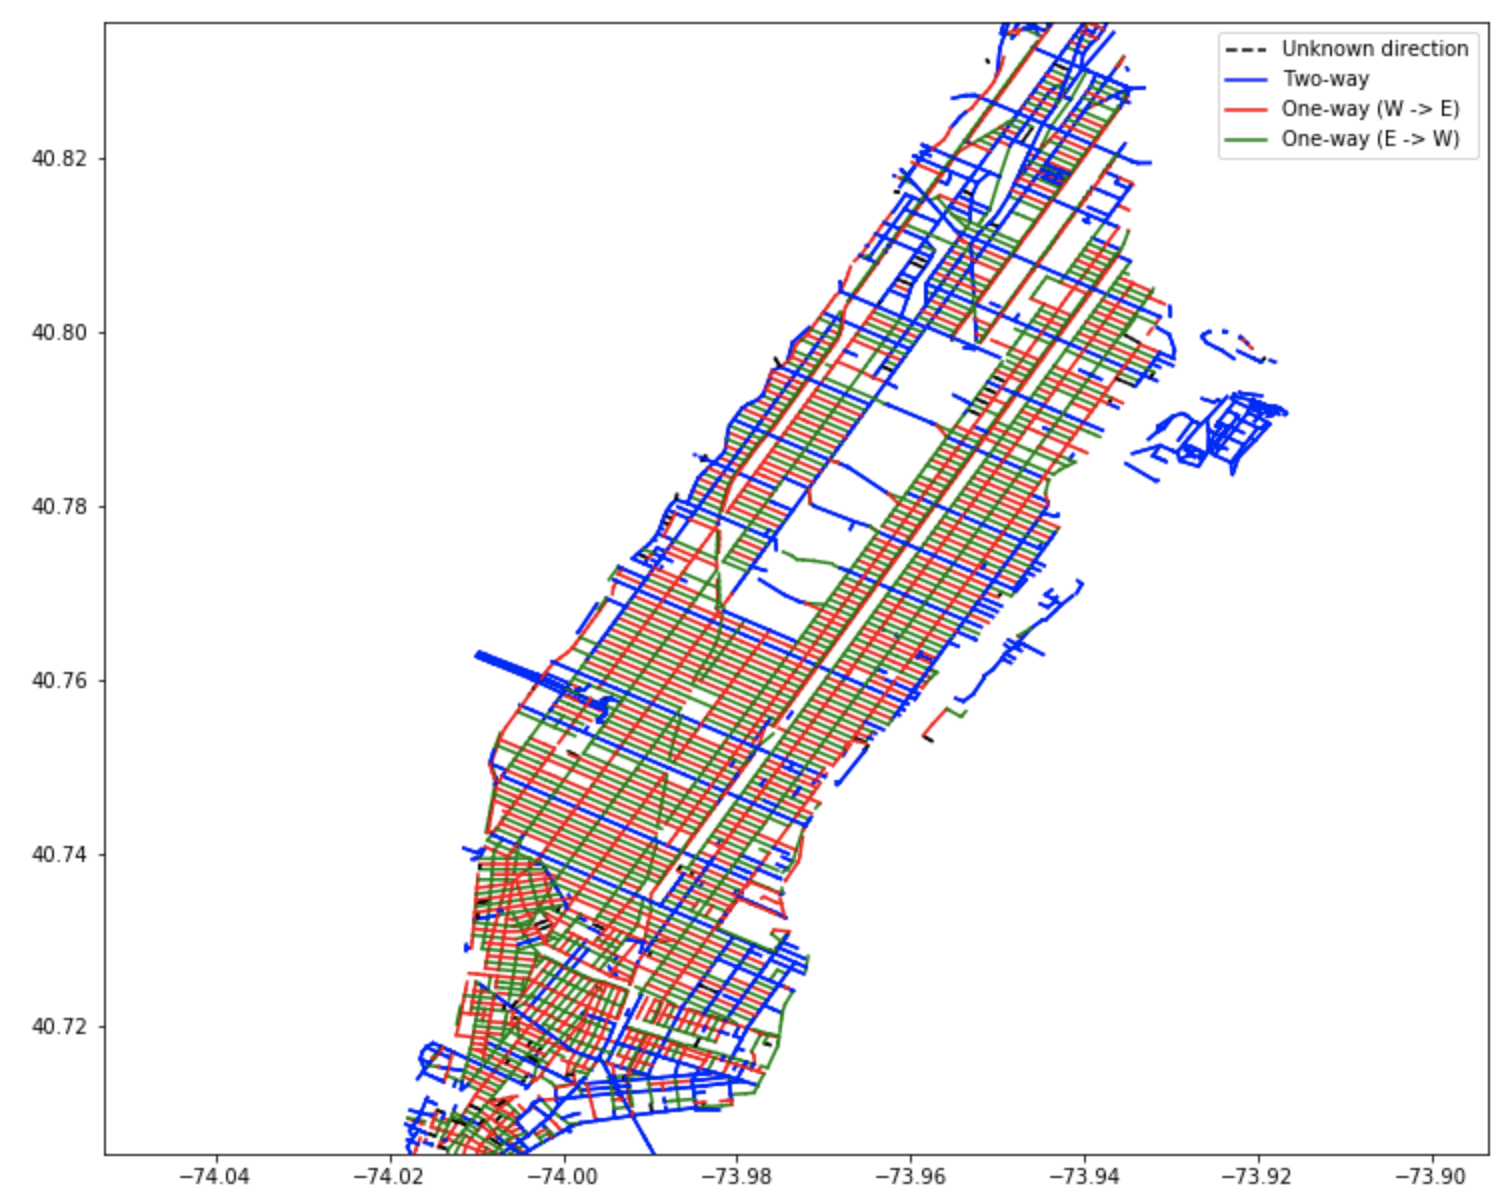
\includegraphics[width=0.7\linewidth]{network.png}
    \caption{Complexity of the Manhattan traffic structure as a graph}
    \label{manhattan}
\end{figure}
Given the complexity of the data---both in the number of parameters we need to fit, as well running graph algorithms on a large network---we have since refined our approach. We now aim to discretize Manhattan into a grid and have latent variables for the congestion within each of these discrete units. (See Section~\ref{results})

\subsection{Evaluation}

In our initial proposal, we suggested an $\ell^2$ norm for penalizing predictions would be natural. Upon further inspection of the data, however, we have realized the distribution of travel times has a very heavy right-tail (some trips apparently taking days). Since these observations are either a product of un-clean data or values which we don't particularly care to predict, we opt for reporting percentiles of the $\ell^2$ norm.

\section{Baseline results}

We have two models as baseline. We use a ridge regression and a neural network on the following set of features: trip distance, day of the week, and hour of the day. For the ridge regression, we observed the estimated coefficients of Wednesday to Friday to be the highest among days of the week, and coefficients of 2am-6am to be significantly lower than other hours of the day.
\begin{center}
\begin{tabular}{ccc}\toprule 
    Test-set error descriptive statistics (minutes) & Ridge regression & Neural network \\\midrule
    Mean & 3.684 & 3.544\\
    Standard deviation & 22.177 & 21.786\\
    99\% percentile & 15.268 & 15.059\\\bottomrule
\end{tabular}
\end{center}
Although the neural network model has marginally better performance than the ridge regression and can arguably improve with further parameter tuning, the coefficients of the ridge regression is much more interpretable and generates useful insights. Our approach in Section~\ref{results} shares this feature with the linear regression in generating interpretable coefficients of interest.


\section{Preliminary results}
\label{results}
We implemented a model based on discretization. Since the discretization of Manhattan into literal streets is too cumbersome, we opt to discretize Manhattan into a $P\times Q$ grid (We believe that $40\times 140$ performs well). To put in perspective, each grid point corresponds to roughly a $200\text{ft} \times 200\text{ft}$ area. We convert the coordinates of start and end locations of each trip to the nearest grid point. Let each grid point be associated with a weight $w_i$ whose collection is $\bm W$. These weights represent expected trip times ``passing through'' a grid point.\footnote{If we discretize Manhattan into actual streets, then each street segment would have a weight that indicates how long it takes for a driver to traverse this street segment. Here, the weight of each grid point gives a general sense of how congested a small patch of land is.} 

Let $G = \{1,\ldots,N\}$ be the set of grid points. Let $\mathcal{Z}_{ij} \subset 2^G$ be the set of paths from $i$ to $j$.
For each trip $k$ starting from $i$ and ending at $j$, let $T_k$ be the time the trip takes. Let $z_k \in \mathcal{Z}_{ij}$ be a latent variable of the path taken by the trip. We have a mixture model 
\begin{align*}
z_k | \bm W &\sim \mathcal{L}_{\mathcal{Z}_{ij}}\\
T_k | z_k &\sim \mathcal{N}\left(\sum_{i\in z_k} w_i, \sigma^2\right),
\end{align*}
where $\mathcal{L}$ is some distribution over $\mathcal{Z}_{ij}$ and $\bm W = (w_i)_i$ are the weights associated with node $i$---which should be an estimate of time it takes to traverse the grid node.

We assume $\mathcal{L}$ is the following. The driver would only traverse in the direction of her destination. Given hyperparameter $q \in [0,1]$, the driver traverses the shortest-time route ($\argmin_{z} \sum_{z} w_i$) with probability $q$ and randomly picks a route in the direction of her destination with probability $1-q$.

We took an approach that is similar to expectation-maximization and to stochastic variational inference. For each observation, we sample from $\mathcal L_{\mathcal Z_{ij}}$ conditional on the \emph{current} estimates of $\bm W$. We then update the parameters $\bm W$ via the gradients of the squared error loss between the predicted trip time and the actual trip time (thus corresponding to a Normal model with known variance). This approach is similar to \cite{zhan2013urban}, who also use a mixture model, while using a discrete choice model for modeling $\mathcal L_{\mathcal Z_{ij}}$. However, the model in \cite{zhan2013urban} runs on a much smaller scale facing larger computational constraints, whereas we are able to estimate on a larger scale by using a sampling approach for $\mathcal L_{\mathcal Z_{ij}}$. 

There are a few interesting results to note:
\begin{enumerate}
    \item The model performs well even with a small dimension of points. In Figure~\ref{errs}, we use a model with only 350 parameters (about 1/5 of the neutral network), we are able to achieve test-set error rates that are on par with the neural net. Moreover, we have not stratified the data by time and week, which are important predictors of trip time in the model.
    \item The visualization of the model is telling. In all three dimensions of the model that we tested (Figure~\ref{small} and Figure~\ref{larger}), the visualization of the model parameters are able to identify similar areas of high and low congestion. This is robust to dimension, initialization, and values of $q$ (Figure~\ref{nosmooth}). 
    \item The model is a bit sensitive to extreme values (which we suspect to be data errors). The extreme values tend to be unusually long trips, and they tend to update the parameters in extreme directions (the red lines in Figures~\ref{larger} and \ref{nosmooth}). Though these errors fade out over time (see attached 100-frame video of visualizations with one frame for 2000 trips\footnote{The images are snapshots of parameter values in the updating process}), they fade out especially slowly since trips that take long are unlikely to be selected if $q$ is high, and thus it's hard for high parameter values to be corrected on later conditioning.
    \item We also observe that $q$ acts as a smoothing parameter. With $q=1$ in Figure~\ref{nosmooth}, the parameters rigid, forming clear lines that probably represents the disproportionate effects of only a few trips.
\end{enumerate}

\subsection{Future directions}
Here are a few areas we are looking to explore:
\begin{itemize}
    \item We are looking to explore the theoretical properties of the model and estimation approach by formalizing them in terms of EM and stochastic variational inference.
    \item We will split the training sample by some observable characteristics such as day of the week and time of day, and train on each subsample. This approach should improve prediction accuracy, and provide more insight in the evolution of congestion in the temporal dimension.
    \item We will consider remedies of extreme values. Currently, since we assume drivers behave intelligently, weights that are overly large (usually due to unusually long trips because of unclean data) tend to very slowly be corrected, since intelligent drivers avoid such routes and prevents the routes from being observed and updated. Graphically, this results in abrupt red lines across our Manhattan map and only updated gradually.
    \item We will attempt to address the intractability of parameter optimization on the exact street network by dividing Manhattan into neighborhoods and optimize the street weights by training on a subsample of the dataset restricted to each neighborhood. With the weight of each streets calculated, we then make prediction on the complete test set.
\end{itemize}

\bibliographystyle{IEEEtran}
\bibliography{refs}

\appendix
\section{Attached figures}

\begin{figure}[!h]
\centering
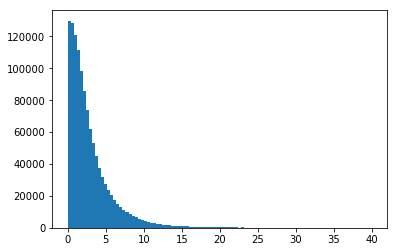
\includegraphics[width=0.7\textwidth]{error.png}
\caption{The distribution of error obtained on the test set by using a low-dimensional model with $P=10, Q = 35$ and $q=1$. The mean loss is $3.28$ minutes and the 99\% is $15.49$ minutes in error.}
\label{errs}
\end{figure}


\begin{figure}[!h]
\centering
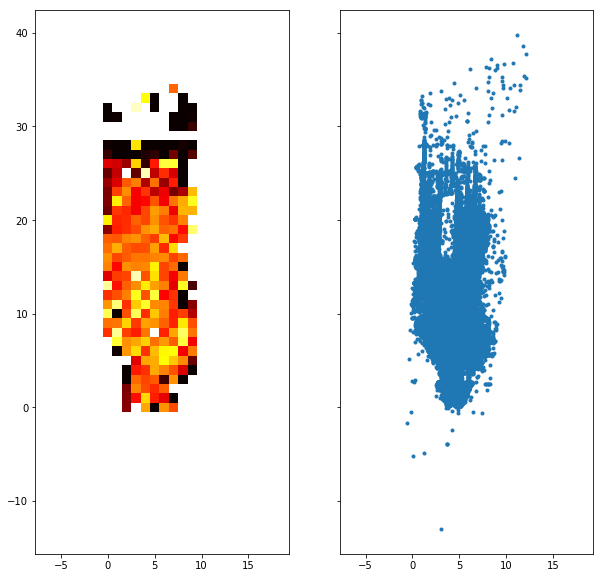
\includegraphics[width=0.7\textwidth]{low-dim1.png}
\caption{We plot via \texttt{plt.imshow(...,cmap='hot')} the distribution of parameter values since they have physical interpretations on a heat map. The right panel is the distribution of trip starting locations which trace out the shape of Manhattan. This is on a low dimensional model with $P=10, Q = 35$. Here, brighter colors (yellow) means higher parameter value, which points to more congestion. We also initialize grid points that are above non-terrestrial areas (e.g. Hudson river) to have high values and omit them in the plotting. We later realized that the initialization does not matter, and the model is able to pick up the shape of Manhattan automatically.}
\label{small}
\end{figure}

\begin{figure}[!h]
\centering
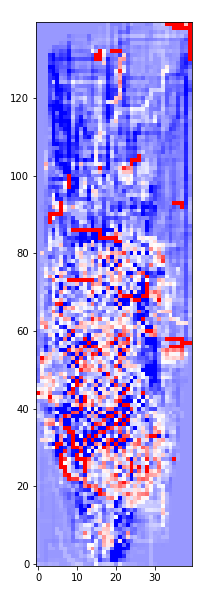
\includegraphics[width=0.4\textwidth]{91.png}
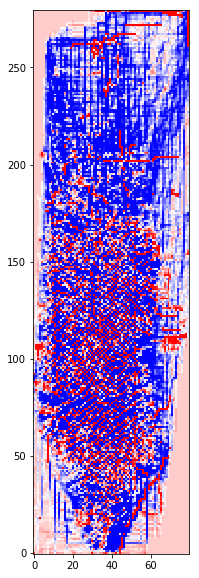
\includegraphics[width=0.39\textwidth]{large.png}
\caption{Left: an iteration of the model with $40 \times 140$ parameters. Right: an iteration of the model with $80\times 280$ parameters. In both, $q=0.5$.}
\label{larger}
\end{figure}

\begin{figure}[!h]
\centering
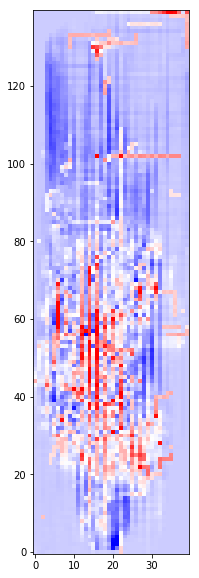
\includegraphics[width=0.4\textwidth]{no_smooth.png}
\caption{An iteration of the model with $q = 1$. We see that without smoothing, the parameters doesn't really look right. }
\label{nosmooth}
\end{figure}

\end{document}


